\section{Diagramme de cas d'utilisation}
	\begin{figure}[H]
		\centering
		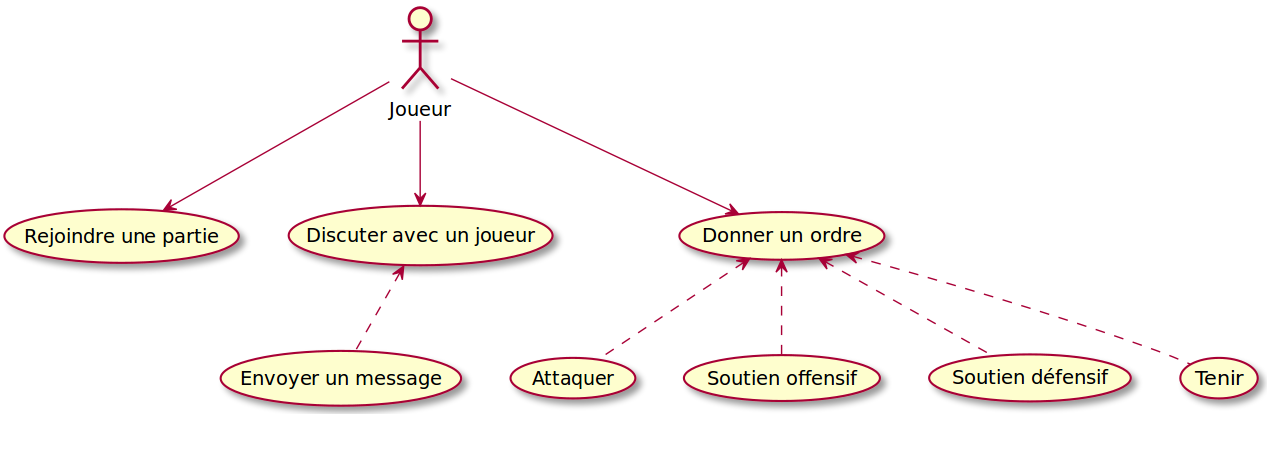
\includegraphics[scale=0.4]{images/UseCase.png}
		\caption{Diagramme de cas d'utilisation}
	\end{figure}


\section{Diagramme de classes participantes}
	\subsection{Partie Serveur}
		\subsubsection{Moteur du jeu}
        Les diagrammes décrivant le moteur du jeu sont les figures \ref{pparties}, \ref{parmees}, \ref{pcartes}, \ref{pjoueurs}, \ref{pmessages}.
			\begin{figure}[H]
				\centering
                \includegraphics[scale=0.7]{diagrammes/php-export-cut/Parties.png}
                \caption{\label{pparties}Package Parties}
			\end{figure}

			\begin{figure}[H]
				\centering
                \includegraphics[scale=0.5]{diagrammes/php-export-cut/Armees.png}
                \caption{\label{parmees}Package Armees}
			\end{figure}

			\begin{figure}[H]
				\centering
                \includegraphics[scale=0.3]{diagrammes/php-export-cut/Cartes.png}
                \caption{\label{pcartes}Package Cartes}
			\end{figure}

			\begin{figure}[H]
				\centering
                \includegraphics[scale=0.45]{diagrammes/php-export-cut/Joueurs.png}
                \caption{\label{pjoueurs}Package Joueurs}
			\end{figure}

			\begin{figure}[h!]
				\centering
                \includegraphics[scale=0.35]{diagrammes/php-export-cut/Messages.png}
                \caption{\label{pmessages}Package Messages}
                \pagebreak
			\end{figure}

        \subsubsection{Les phases du jeu}
        Le diagramme décrivant les phases du jeu est visible dans la figure~\ref{pphases}.

			\begin{figure}[H]
				\centering
                \includegraphics[scale=0.7]{diagrammes/php-export-cut/Phases.png}
                \caption{\label{pphases}Package Phases}
			\end{figure}

        \subsubsection{Les contrôleurs HTTP}
        Le diagrammes décrivant le package \verb|Http.Controllers| étant trop grand, il est consultable à l'URL \url{https://diplo-lejeu.fr/images/http\_controllers.png}.

        \subsubsection{Les événements}
        Les diagrammes décrivant les événements et la gestion de ceux-ci sont visibles dans les figures \ref{pevents}, \ref{phandlers}, \ref{pcommands}.

        	\begin{figure}[H]
				\centering
                \includegraphics[scale=0.4]{diagrammes/php-export-cut/Events.png}
                \caption{\label{pevents}Package Events}
			\end{figure}

			\begin{figure}[H]
				\centering
                \includegraphics[scale=0.25]{diagrammes/php-export-cut/Handlers.png}
                \caption{\label{phandlers}Package Handlers}
			\end{figure}

			\begin{figure}[H]
				\centering
                \includegraphics[scale=0.7]{diagrammes/php-export-cut/Commands.png}
                \caption{\label{pcommands}Package Commands}
			\end{figure}

        \subsubsection{Les Service Providers}
        Le diagrammes décrivant les Service Providers, propres au framework Laravel est visible dans la figure~\ref{pproviders}.

			\begin{figure}[H]
				\centering
                \includegraphics[scale=0.4]{diagrammes/php-export-cut/Providers.png}
                \caption{\label{pproviders}Package Providers}
			\end{figure}

		\subsubsection{Les ordres}
        Le diagrammes décrivant les ordres du jeu étant trop grand, il est consultable à l'URL suivante \url{https://diplo-lejeu.fr/images/ordres.png}

		\subsubsection{Les exceptions}
        Les diagrammes décrivant les exceptions du jeu étant trop grand, il est consultable à l'URL suivante \url{https://diplo-lejeu.fr/images/exceptions.png}

    \pagebreak
	\subsection{Partie Client}

\section{Diagramme de packages}
	\subsection{Partie Serveur}
		\subsubsection{Première partie}
			\vspace{10mm}
			\begin{figure}[H]
				\centering
				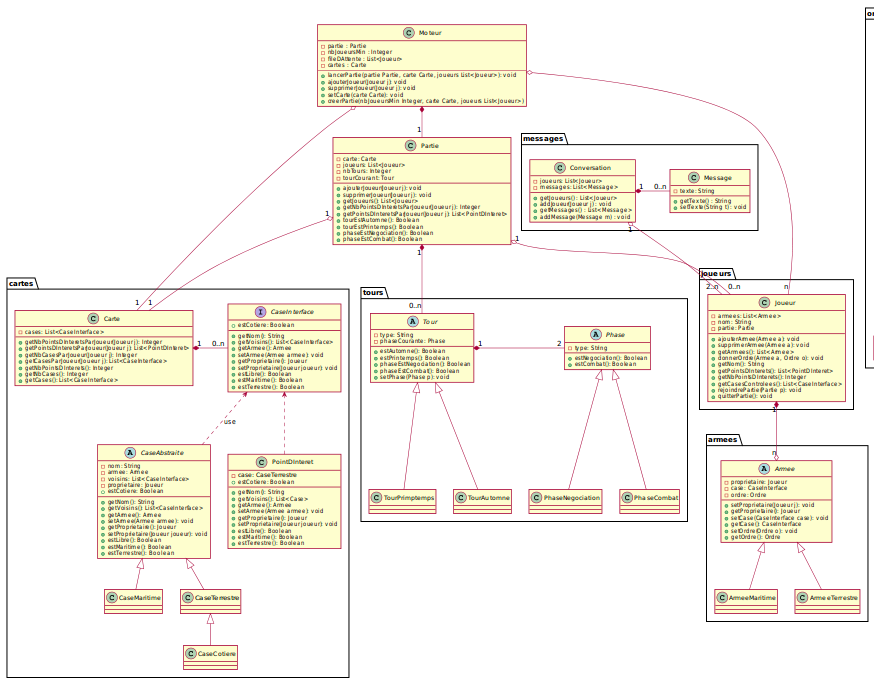
\includegraphics[angle=90,width=150mm]{images/DP1.png}
				\caption{Première partie}
			\end{figure}


		\subsubsection{Deuxième partie}
			\vspace{10mm}
			\begin{figure}[H]
				\centering
				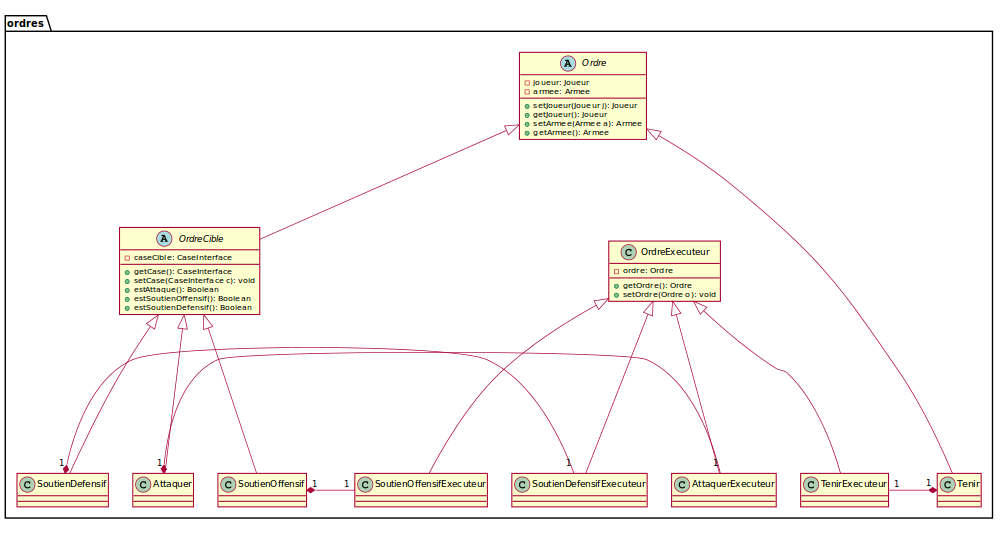
\includegraphics[scale=0.4]{images/DP2.png}
				\caption{Le package Ordres}
			\end{figure}

		\subsubsection{Troisième partie}
			\vspace{10mm}
			\begin{figure}[H]
				\centering
				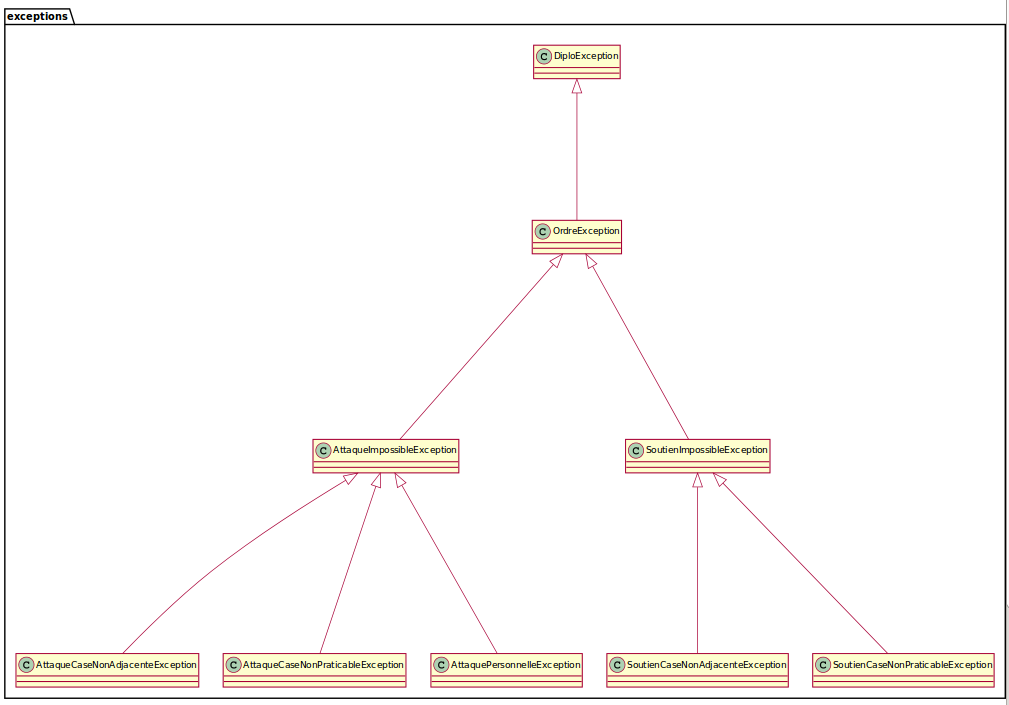
\includegraphics[scale=0.4]{images/DP3.png}
				\caption{Le package Exceptions}
			\end{figure}

	\subsection{Partie Client}

\section{Diagramme de séquence système}
	\subsection{Créer une partie}
		\vspace{10mm}
		\begin{figure}[H]
			\centering
			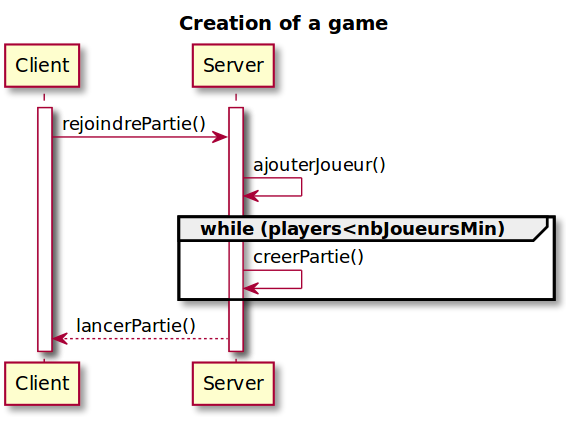
\includegraphics[scale=0.5]{images/DSSCreate.png}
			\caption{Créer une partie}
		\end{figure}

	\subsection{Jouer son tour}
		\vspace{10mm}
		\begin{figure}[H]
			\centering
			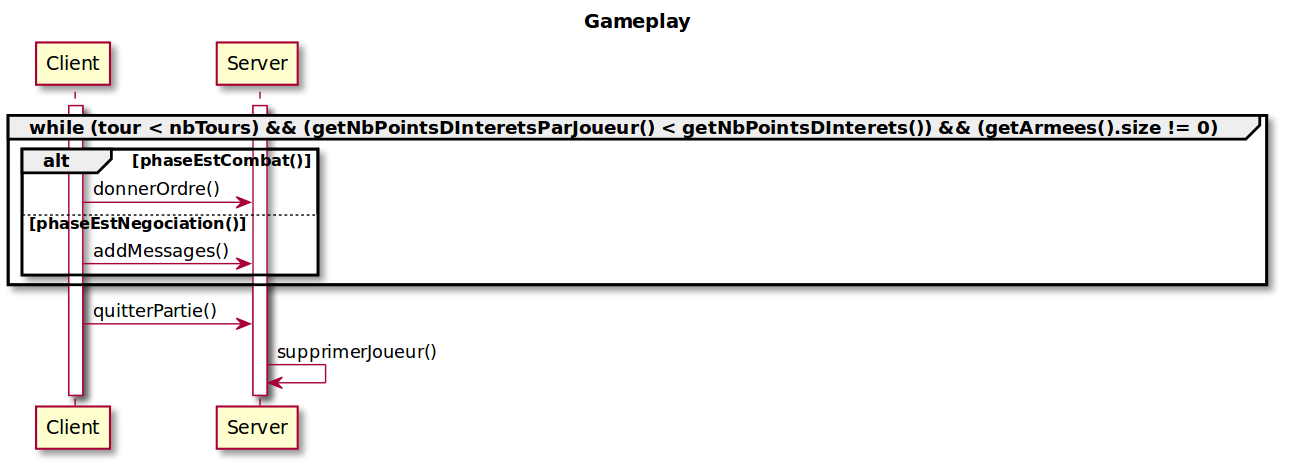
\includegraphics[scale=0.3]{images/DSSGameplay.png}
			\caption{Jouer son tour}
		\end{figure}
		\vspace{70mm}

\section{Sources du DCP et du diagramme de package}
	\begin{itemize}
		\item DCP : \url{http://goo.gl/7uLQP4}
		\item Diagramme de Package : \url{http://goo.gl/LsiHrs}
	\end{itemize}
